% Template for Cogsci submission with R Markdown

% Stuff changed from original Markdown PLOS Template
\documentclass[10pt, letterpaper]{article}

\usepackage{cogsci}
\usepackage{pslatex}
\usepackage{float}
\usepackage{caption}

% amsmath package, useful for mathematical formulas
\usepackage{amsmath}

% amssymb package, useful for mathematical symbols
\usepackage{amssymb}

% hyperref package, useful for hyperlinks
\usepackage{hyperref}

% graphicx package, useful for including eps and pdf graphics
% include graphics with the command \includegraphics
\usepackage{graphicx}

% Sweave(-like)
\usepackage{fancyvrb}
\DefineVerbatimEnvironment{Sinput}{Verbatim}{fontshape=sl}
\DefineVerbatimEnvironment{Soutput}{Verbatim}{}
\DefineVerbatimEnvironment{Scode}{Verbatim}{fontshape=sl}
\newenvironment{Schunk}{}{}
\DefineVerbatimEnvironment{Code}{Verbatim}{}
\DefineVerbatimEnvironment{CodeInput}{Verbatim}{fontshape=sl}
\DefineVerbatimEnvironment{CodeOutput}{Verbatim}{}
\newenvironment{CodeChunk}{}{}

% cite package, to clean up citations in the main text. Do not remove.
\usepackage{cite}

\usepackage{color}

% Use doublespacing - comment out for single spacing
%\usepackage{setspace}
%\doublespacing


% % Text layout
% \topmargin 0.0cm
% \oddsidemargin 0.5cm
% \evensidemargin 0.5cm
% \textwidth 16cm
% \textheight 21cm

\title{Balancing informational and social goals in active learning}


\author{{\large \bf Erica J. Yoon*}, {\large \bf Kyle MacDonald*}, {\large \bf Mika Asaba}, {\large \bf Hyowon Gweon}, \and {\large \bf Michael C. Frank} \\ \{ejyoon, kylem4, masaba, hyo, mcfrank\} @stanford.edu \\ Department of Psychology, Stanford University \\ *These authors contributed equally to this work.}

\begin{document}

\maketitle

\begin{abstract}
Our actions shape what we learn. Because of this dependency, learners
are proficient at choosing their actions to maximize their information
gain. But learning often unfolds in social contexts where learners have
both informational goals (e.g., to learn how something works) but also
social goals (e.g., to appear competent and impress others). How do
these different factors shape learners' decisions? Here, we present a
computational model that integrates the value of social and
informational goals to predict the decisions that people will make in a
simple active causal learning task. We show that an emphasis on
performance or self-presentation goals leads to reduced chances of
learning (Exp. 1) and that social context can push learners to pursue
performance-oriented actions even when the learning goal is highlighted
(Exp. 2). Our formal model of social-active learning successfully
captures the empirical results. These findings are first steps towards
understanding the role of social reasoning in active learning contexts.

\textbf{Keywords:}
active learning; social reasoning; information gain; OED;
self-presentation; goal tradeoffs
\end{abstract}

\section{Introduction}\label{introduction}

Imagine you are a novice cook and you have to decide what meal to
prepare for a first date. Should you choose an easy favorite or attempt
to make something new? While the familiar recipe can ensure a good meal,
you may miss out on a new, delicious dish. The new recipe might taste
even better, but it has a higher chance of failure. In this type of
\emph{explore-exploit} dilemma (Sutton \& Barto, 1998), you can choose
between \emph{exploring} the new recipe that may or may not result in a
more delicious dish (\emph{learning} goal), or \emph{exploiting} your
previous experience and knowledge to ensure a good meal
(\emph{performance} goal). Here, we explore the idea of formalizing the
learning-performance goal tradeoff using a simple active learning
context, where social factors may shape the goals we consider.

Active learning occurs when people have control over the sequence of
information in a learning context (e.g., press buttons on a toy, one by
one, to see their effect). The key assumption of this framework is that
learners maximize the utility of their actions by gathering information
that is especially helpful for their own learning. Empirical work in
education (Grabinger \& Dunlap, 1995), machine learning (Settles, 2012),
and cognitive psychology (Castro et al., 2009) suggests that active
contexts lead to faster learning than passive contexts where people
don't have control over the information flow.

But real-world learning usually takes place in rich social contexts with
teachers, peers, or other people who can directly influence our
learning. Indeed, adults and even preschool-aged children modulate their
inferences depending on how others (e.g., teachers) select their actions
(Shafto, Goodman, \& Frank, 2012), and understand that socially
communicated information licenses different inferences than information
generated on their own (e.g., Xu \& Tenenbaum, 2007). But even when we
learn from \emph{our} own actions instead of others', our social
environment may affect our self-directed learning process. While
previous models have captured how we optimize learning, either from our
own actions or from others, they have been agnostic to other social
factors that are ubiquitous in a learner's environment. People must
integrate the value of social goals (e.g., looking competent or
knowledgeable) and informational goals when deciding what to do.

How can active learning models accommodate this richer set of utilities?
As a step towards answering this question, we model a learner who
considers a mixture of learning and performance goals. A key assumption
underlying recent Bayesian models of human social cognition is that
people expect others to act approximately optimally given a utility
function (e.g., Goodman \& Frank, 2016; Jara-Ettinger, Gweon, Schulz, \&
Tenenbaum, 2016). Our model adopts this utility-theoretic approach, and
assumes an agent who reasons about the utility function that represents
a weighted combination of multiple goals (Yoon, Tessler, Goodman, \&
Frank, 2017) in a social active learning context.\footnote{Such models
  are commonly used to approximate group-level behavior, without the
  strong assumption that individuals must be strictly optimal (e.g.,
  Frank, 2013; Goodman et al., 2015).}

\begin{CodeChunk}
\begin{figure}[b]

{\centering 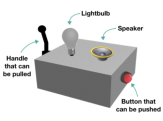
\includegraphics[width=0.65\linewidth]{figs/toy-1} 

}

\caption[An example of the toy used in our paradigm]{An example of the toy used in our paradigm.}\label{fig:toy}
\end{figure}
\end{CodeChunk}

\begin{CodeChunk}
\begin{figure*}[tb]

{\centering 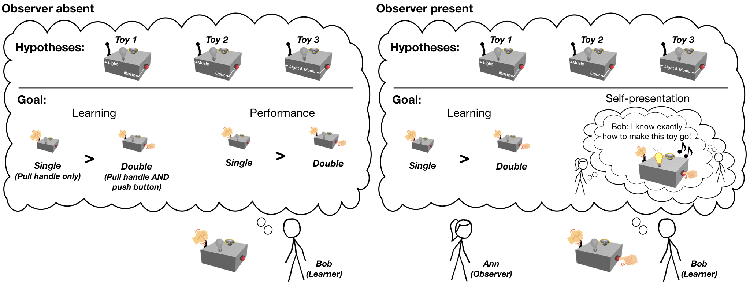
\includegraphics[width=0.95\linewidth]{figs/model_diagram-1} 

}

\caption[Model schematic for the learner's inference]{Model schematic for the learner's inference. The learner considers possible hypotheses: Toy 1 (handle pull turns on the light, button press turns on music, both actions cause both effects); Toy 2 (handle pull turns on music, button press turns on the light, both actions cause both effects); and Toy 3 (both actions cause both effects, but each action on its own does not produce any effect). The learner also considers his goals. When an observer is absent, he considers his learning goal and performance goal and chooses an action. The learning goal favors a ``single" action (e.g., pull the handle only) that can fully disambiguate, whereas the performance goal favors the ``both" action (pull the handle AND push the button) that guarantees the most salient reward. When an observer is present, the learner considers the learning, performance (not shown), and self-presentation goal.}\label{fig:model_diagram}
\end{figure*}
\end{CodeChunk}

We instantiate our model in a simple causal learning task and examine
how people choose actions that support learning vs.~performance goals in
different social contexts. We present a toy with an ambiguous causal
mechanism (Fig.~\ref{fig:toy}). For this toy, doing only one of the two
possible actions (handle pull or button press) disambiguates its causal
mechanism but potentially risks no immediate effect (i.e., neither sound
nor light turning on), while doing both actions at the same time is
immediately rewarding (both music and light on) but is not informative
for learning the toy's causal mechanism. Thus, the learner can choose
between the two actions that will each lead to either a new discovery
(exploration; learning) or an immediate reward (exploitation;
performance). The learner's action rests on relative utilities he
assigns to learning versus performance, which in turn are determined in
part by the social context (e.g., the presence or absence of his
boss).\footnote{From here on, we use a male pronoun for Bob, the learner, and female pronoun for Ann, the boss and observer.}

In two experiments, we show that emphasizing performance or
self-presentation (social) goals leads to actions that are not
informative and thus reduces the chances of learning (Exp.~1). Next, we
show that the mere presence of an observer (i.e., a boss) pushes
learners to consider performance/presentation-oriented actions even when
the learning goal is highlighted (Exp.~2). Finally, we show that the
empirical results are consistent with predictions of our cognitive model
of social-active learning.

\section{Computational model}\label{computational-model}

We model a learner \(L\) who chooses his action \(a\) approximately
optimally (as per optimality parameter \(\lambda\)) based on the
expected total utility \(U_{t}\) given his action and presence of an
observer \(o\):

\[ P_L(a | o) \propto \exp(\lambda \cdot \mathbb{E}[U_{t}(a,o)]).\]
\noindent
The total utility is defined as:
\[U_{t}(a,o) = \phi_{learn} \cdot U_{learn}(a) + \phi_{perf} \cdot U_{perf}(a) + \delta^o \cdot \phi_{pres} \cdot U_{pres}(a),\]
\noindent
where \(\phi\)s are weights that are inferred for each utility from data
and \(\delta^o\) is a Dirac delta function that is 1 if there is an
observer, and 0 if there is no observer. Below we describe the structure
of each utility (see Fig.~\ref{fig:model_diagram} for the model
schematic).

\subsubsection{Learning utility}\label{learning-utility}

The \emph{learning utility} captures the goal to learn new information,
which in our paradigm is associated with figuring out how a given toy
works. The learning utility (\(U_{learn}\)) in our model is derived from
Optimal Experiment Design models (OED; Nelson, 2005), which quantify the
expected utility of different information seeking actions. The learner
is uncertain about the mechanism of toy \(t\) and wants to decrease his
uncertainty by taking an action. This decrease is captured by
\emph{information gain} due to an action, the change in the learner's
entropy (uncertainty) before and after seeing an outcome of the action.
To maximize information gain, the learner sums the information gain due
to each outcome \(m\) in the set of possible outcomes \(M\) (e.g., music
playing), weighted by the probability of that outcome given the action.
Thus,
\[ U_{learn}(a) \propto \sum_{m \in M}{P(m|a)}[{H(t) - H(t | m,a)}],\]
\noindent
where \(H(t)\) is the Shannon entropy of the learner's guess about the
toy (MacKay, 2003). Once the learner chooses an action and observes an
outcome, then he updates his beliefs about each hypothesis via standard
Bayesian updating. Finally, we scale the utility by \(log_2n\), where
\(n\) is the number of possible actions, to convert the utility to a
value between 0 and 1.

\subsubsection{Performance utility}\label{performance-utility}

The \emph{performance utility} is the utility of achieving an immediate
rewarding outcome. Within our paradigm, the learner gains utility from
an immediate effect of music or light turning on. The expected
performance utility (\(U_{perf}\)) before the learner chooses an action
is the likelihood of an effect \(m\) given the action \(a\):
\[ U_{perf}(a) = P_L(m | a).\] \noindent

\subsubsection{Presentation utility}\label{presentation-utility}

When there is another person present to observe the learner's action,
the observer \(O\) is expected to reason about the learner \(L\)'s
competence, equal to whether the learner was able to make the toy
produce an effect. The learner thinks about the observer's inferential
process, and the expected \emph{presentation utility} (\(U_{pres}\)) is
based on maximizing the apparent competence inferred by the observer:
\[ U_{pres}(a) = P_O(m | a),\] \noindent
where \(P_O(m | a)\) is the observer's own estimate of the likelihood of
an effect given the learner's action.\footnote{We assume that the
  observer is naive about the toy's causal structure; if the observer is
  knowledgeable, \(U_{perf}\) and \(U_{pres}\) will diverge, which is an
  important consideration for future work.}

\section{Experiment 1}\label{experiment-1}

In Experiment 1 (Exp.~1), we first wanted to confirm that participants
would choose different actions depending on what goal was highlighted.
We were also interested in how people would act when no explicit goal
was specified within the task. Participants were asked to act on a toy
with an ambiguous causal structure, and were assigned to different goal
conditions: (1) Learning (i.e., learn how the toy works), (2)
Performance (e.g., make the toy play music), (3) Presentation (i.e.,
impress their boss), and (4) No goal specified. We hypothesized that
participants would choose an informative action more often in the
following order of goal conditions (decreasing): Learning, No-goal,
Performance, and
Presentation.\footnote{Our hypothesis, method, model and data analysis were pre-registered prior to data collection at \url{https://osf.io/kcjau}.}

\subsection{Method}\label{method}

\subsubsection{Participants}\label{participants}

We recruited 196 participants (45-51 per condition) on Amazon's
Mechanical Turk, with IP addresses in the US and a task approval rate
above 85\%. We excluded 7 participants who failed to answer at least two
out of three manipulation check questions correctly (see Procedure
section for details on the manipulation check), and thus the remaining
189 participants were included in our final analysis.

\subsubsection{Stimuli and Design}\label{stimuli-and-design}

We presented images and instructions for three different toys that
looked very similar but worked in different ways (see captions for
Fig.~\ref{fig:model_diagram}). The instructions conveyed that pressing
the button and pulling the handle at the same time was immediately
rewarding but uninformative (fails to disambiguate the causal
mechanism). In contrast, either of the single actions was completely
disambiguating, but was uncertain to produce an immediate outcome. Each
toy had a label at the front, indicating the correct action(s)--outcome
link.

\begin{CodeChunk}
\begin{figure}[H]

{\centering 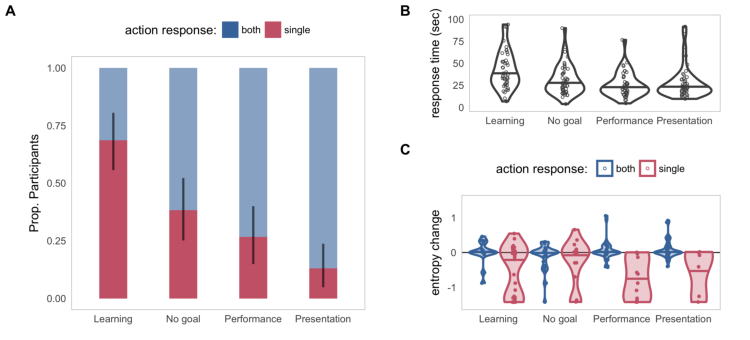
\includegraphics[width=0.86\linewidth]{figs/e1_behav_results_plot-1} 

}

\caption[Behavioral results for Exp]{Behavioral results for Exp. 1. A: Proportion of action decisions for each goal condition. Error bars are 95\% binomial CIs based on a Bayesian beta-binomial model. B: Distribution of response times on the action decisions. C: Distribution of participants' belief change (information gain in bits) as a function of condition. Higher values represent more information gained from the action selection.}\label{fig:e1_behav_results_plot}
\end{figure}
\end{CodeChunk}

We asked participants to act on one of these toys; importantly, the
given toy was missing its label, leading to uncertainty about its causal
structure. We randomly assigned participants into four goal conditions.
In the \emph{No-goal} condition we did not specify any goal for
participants. In the \emph{Learning}, \emph{Performance}, and
\emph{Presentation} conditions, we asked participants to imagine they
were toy developers and one day their boss approached them. We
instructed participants to: figure out the correct label for the toy
(\emph{Learning}); make the toy play music (or turn the light on;
\emph{Performance}); or impress their boss and show that they are
competent (\emph{Presentation}). We asked participants to select an
action out of the following set: ``press the button'', ``pull the
handle'', or ``press the button and pull the handle.'' The order of
actions was randomized.

\subsubsection{Procedure}\label{procedure}

In the \emph{exposure phase}, we showed participants an example toy and
gave instructions for three toy types. We first presented the
instructions for the single action toys (Toy 1 and Toy 2) in a
randomized order, and then presented the instructions for the both
action toy (Toy 3). After instructions, participants indicated what
action would make each toy operate (e.g., ``How would you make
{[}this{]} toy play music?'') to show that they understood how the
different toys worked.

In the \emph{test phase}, participants read a scenario for one of the
four goal conditions, followed by the question: ``If you only had one
chance to try a SINGLE action {[}to pursue the specified goal{]}, which
action would you want to take? You will get a 10 cent bonus \ldots{} if
you {[}achieve the given goal{]}''.

Both before and after the critical action decision trial, we asked
participants to rate the likelihood that the unknown toy was Toy 1, 2,
or 3, which indexed participants' prior beliefs about how the toys were
likely to function and their \emph{belief change} after selecting an
action and observing its effect.

\subsection{Results and discussion}\label{results-and-discussion}

\subsubsection{Action decisions:}\label{action-decisions}

We modeled action decisions using a logistic regression
\texttt{$action \sim goal\_condition$} with the No-goal condition as the
reference
category.\footnote{In all of the analyses for Exp.\ 1 and Exp.\ 2, we used the {\fontfamily{qcr}\selectfont rstanarm} package to fit Bayesian regression models estimating the differences across conditions. We report the uncertainty in our point estimates using 95\% Highest Density Intervals (HDI). The HDI provides a range of credible values given the data and model.}
Participants' tendency to select a ``single'' action (button press or
handle pull, each on its own) varied across conditions as predicted
(Fig.~\ref{fig:e1_behav_results_plot}A), with the highest proportion in
the Learning condition, followed by No-goal, Performance, and
Presentation.

Compared to the No-goal condition, participants selected the single
action at a greater rate in the Learning condition (\(\beta\) = 1.18,
{[}0.82, 1.55{]}) and at lower rate in the Presentation context
(\(\beta\) = -1.53, {[}-2, -1.06{]}), with the null value of zero
difference condition falling well outside the 95\% HDI, and at similar
rate in the Performance condition (\(\beta\) = -0.65, {[}-1.04,
-0.27{]}) with the 95\% HDI including the null.

\subsubsection{Action decision times:}\label{action-decision-times}

We analyzed decision times, which were the latency to make an action
selection as measured from the start of the action decision trial (all
RTs were analyzed in log space), using the same model specification as
action decisions. Fig.~\ref{fig:e1_behav_results_plot}A shows the full
RT data distribution. Compared to the No-goal condition, participants
took longer to generate a decision in the Learning condition. In
contrast, participants in the Performance and Presentation conditions
produced similar decision times.

\subsubsection{Belief change:}\label{belief-change}

We quantified participants' change in beliefs about the toy using
information gain. We computed the Kullback-Leibler (KL) divergence both
before and after participants' action selections. The KL divergence
gives a measure of the distance between the correct\footnote{Note that
  since the action-effect link was deterministic, the correct belief
  distribution is a function of participant's action decision. For
  example, if a participant selected the button action, then
  \(B_{correct}\) placed 100\% of the probability mass on the button
  hypothesis.} probability distribution and the participant's beliefs
about the identity of the unlabeled toy. We notate participants' belief
distributions as \(B_{prior}\) and \(B_{prior+a}\) and the correct
distribution as \(B_{correct}\). The difference between these KL
divergences provides the number of bits of information gained due to the
action:
\(IG(a) = D_{KL} ( B_{correct}|| B_{prior} ) - D_{KL} (B_{correct} || B_{prior+a} )\).

We modeled information gain as a function of goal condition and action
choices: \texttt{$IG \sim goal\_condition + action\_response$}
(Fig.~\ref{fig:e1_behav_results_plot}C). Across all conditions, people
who selected the single action showed a greater gain in bits of
information (\(\beta_{single}\) = 0.91, {[}0.77, 1.05{]}, i.e., learned
more from their action. We did not see evidence of an interaction
between goal and action selection. However, a larger proportion of
participants selected a single action in the Learning context, so
learning was more likely in this condition.

\section{Experiment 2}\label{experiment-2}

In Exp.~1, we confirmed that participants selected different actions
depending on the type of goal emphasized. In Exp.~2, our goals were
three-fold: (1) to replicate the results from Exp.~1; (2) to manipulate
goals \emph{and} the presence/absence of another person
(social/no-social) independently, allowing us to measure the interaction
between goals and social context; and (3) to compare empirical data with
predictions of our computational model. Our key behavioral prediction
was an interaction: that participants would be less likely to select a
single (more informative) action in the Learning goal and No-goal
conditions when their boss was present. We also predicted a null result:
that the presence of the boss should not affect action decisions in the
Performance condition.

\subsection{Method}\label{method-1}

\subsubsection{Participants}\label{participants-1}

Using the same recruitment and exclusion criteria as Exp.~1, we
recruited 347 participants (42-51 per condition), and included 325
participants in our final analysis.

\subsubsection{Stimuli and Design}\label{stimuli-and-design-1}

The stimuli and design were identical to Exp.~1, except we had 7
different goal \(\times\) social conditions. Goals were identical to
Exp.~1; social context varied depending on whether the boss was present
(\emph{Social}) or absent (\emph{No-social}) in the story. The
conditions were: \emph{Social-learning}, \emph{Social-performance},
\emph{Social-presentation}, \emph{No-social-no-goal},
\emph{No-social-learning}, \emph{No-social-performance}, and
\emph{Social-no-goal}. Note that we did not have
\emph{No-social-presentation} condition, because the presentation goal
was defined by presenting oneself as competent to another person.

\subsubsection{Procedure}\label{procedure-1}

The procedure was identical to Exp.~1.

\subsection{Results and discussion}\label{results-and-discussion-1}

\subsubsection{Action decisions:}\label{action-decisions-1}

We modeled action decisions using a logistic regression specified as
\texttt{$action \sim goal\_condition * social\_context$} with the
No-social-no-goal condition as the reference category. We replicated the
key finding from Exp.~1: participants selected a ``single'' action more
often in the Learning goal condition, followed by the No-goal,
Performance, and Presentation conditions (Fig.~\ref{fig:e2_results}A).
There was a main effect of social context, with participants being less
likely to select the single action when their boss was present
(\(\beta =\) -0.521, {[}-1.005, -0.053{]}). Finally, there was evidence
for a reliable interaction between goal condition and social context
such that the effect of social context was present in the Learning and
No-goal conditions, but not in the Performance condition (\(\beta\)
\(_{int}\) = 1.148, {[}0.049, 2.296{]}).

\subsubsection{Action decision times:}\label{action-decision-times-1}

We replicated the key decision time finding from Exp.~1, with
participants making slower decisions in the Learning context as compared
to Performance/Presentation. On average, participants took 39.32 seconds
to generate a response in the No-goal condition and 40.72 seconds in the
Learning condition. In contrast, decisions were faster in the
Performance (\(\beta\) = -7.67 sec, {[}-14.01, -1.25{]}) and
Presentation (-10.66 seconds, {[}-18.37, -3.36{]}) conditions, which
were similar to one another (Fig.~\ref{fig:e2_results}B). There was no
evidence of a main effect of social context or an interaction between
goal condition and social context. Note that here we did not see a
difference in decision times between the Learning and No-goal
conditions, which is different from the pattern in Exp.~1.

\subsubsection{Belief change:}\label{belief-change-1}

We replicated the information gain effect from Exp.~1: Participants who
selected a single action showed greater information gain across all
conditions (\(\beta_{single}\) = 0.63, {[}0.4, 0.86{]}. There was no
evidence of a main effect of social context or two-/three-way
interactions between social context, goal, and action choice. As in
Exp.~1, more participants selected the single action in the Learning
condition, especially in the No-social context, meaning information gain
was most likely in this learning context.

\subsubsection{BDA model-data fit:}\label{bda-model-data-fit}

In our paradigm, participants chose an action based on a certain
goal.\footnote{For action priors, we used a separate task in which people indicated the likelihood for selecting an action without any information about possible hypotheses or goals. We used the mean likelihood for each action choice as baseline priors in our model.}
We assumed that the goal descriptions (e.g., ``impress your boss'')
conveyed to the participants a particular set of goal weights
\{\(\phi_{learn}\), \(\phi_{perf}\), \(\phi_{pres}\)\} used to generate
action choices. We put uninformative priors on these weights
(\(\phi \sim Unif(0,1)\)) and inferred their credible values for each
social-goal condition, using Bayesian data analytic techniques (Lee \&
Wagenmakers, 2014).

The inferred goal weights were consistent with what we predicted
(Fig.~\ref{fig:e2_results}D). \(\phi_{learn}\) was highest for the
No-social learning condition, whereas the \(\phi_{perf}\) and
\(\phi_{pres}\) together made up the highest portion in the Presentation
condition, with high social pressure to appear competent compared to
other conditions.

We also inferred another parameter of the cognitive model, the
optimality parameter \(\lambda\). We put uninformative prior on the
parameter (\(\lambda \sim Unif(0,10)\)) and inferred its posterior
credible value from the data. We ran 4 MCMC chains for 100,000
iterations, discarding the first 50,000 for burnin. The Maximum A-
Posteriori (MAP) estimate and 95\% Highest Probability Density Interval
(HDI) for \(\lambda\) was 4.79 {[}3.96, 6.2{]}.

\begin{CodeChunk}
\begin{figure}[H]

{\centering 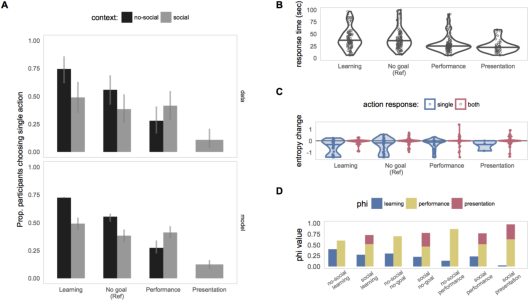
\includegraphics[width=0.95\linewidth]{figs/e2_results-1} 

}

\caption[Behavioral and model results for Exp]{Behavioral and model results for Exp. 2. A: Action decisions from human data (top) and fitted model predictions (bottom). Color represents social context. B and C: Decision times and belief change respectively, collapsing across social contexts. D: Inferred phi values for each condition. All other plotting conventions are the same as Fig. 3.}\label{fig:e2_results}
\end{figure}
\end{CodeChunk}

The fitted model predictions of action choices are shown in
Fig.~\ref{fig:e2_results}A (bottom). The model's expected posteriors
over action choices capture key differences between conditions: the
single action was more likely for No-social than Social conditions
overall, but not when the performance goal was highlighted. The model
was able to predict the distribution of action responses with high
accuracy \(r^2(21)\) = 0.9.

\section{General Discussion}\label{general-discussion}

How do social contexts shape active learning? We proposed that people
integrate informational vs.~social goals when deciding what to do. In
two experiments, we showed that people chose more informative actions
when learning goals were highlighted and in the absence of a relevant
social context (no boss present), while they chose more immediately
rewarding actions when performance/presentational goals were
highlighted, especially when a boss was present. When no goal was
specified, people's behavior seemed to reflect a mixture of goals. Our
model of social-active learning successfully captured key patterns in
the people's action decisions.

This work begins to bring active learning accounts into contact with
social learning theories. We used ideas from Optimal Experiment Design,
which models active learning as a process of rational choice to maximize
information gain, and Rational Speech Act models, which formalize
recursive social reasoning within a Bayesian framework. We included
social information within a formal utility-theoretic framework, building
a richer utility function that represented a weighted combination of
multiple goals -- informational and social.

There are limitations to this work that present opportunities for future
work. First, we did not differentiate between performance and
presentation goals, since the choice of doing both actions satisfies
both of these goals in our paradigm. Enriching the space of possible
actions could tease apart actions driven by self-presentation. Second,
we used a particular social context (the presence of a boss) to
emphasize presentational goals. Our model can be extended to explain a
richer set of social considerations, such as other kinds of observers
(e.g., a teacher who wants the learner to select actions that help her
learn). Third, we limited people to a single action choice. While this
allowed a clean measurement of our condition manipulations, real-world
learning often involves sequential decision-making that could cause
learners to prioritize different goals depending on their prior actions
or the probability of interacting with an observer in the future.

Another interesting open question is how our model could be used to
understand active learning over development. Our framework could allow
us to measure changes in children's goal preferences as they develop
better social reasoning and meta-cognitive abilities. One prediction is
that young children focus on learning goals earlier on when they are
surrounded by familiar caregivers who scaffold learning-relevant
actions. But as their social reasoning abilities mature and their social
environments become more complex, children may start to emphasize
performance or presentation goals.

Overall, this work represents a first step to answering these rich
questions that ultimately seek to unify theories on active learning and
social reasoning.

\vspace{1em}
\fbox{\parbox[b][][c]{7.3cm}{\centering All experiments, data, model, and analysis codes are available in the public repository for the project: \url{https://github.com/kemacdonald/soc-info}}}
\vspace{1em} \noindent

\section{Acknowledgements}\label{acknowledgements}

This work was supported by an NSERC postgraduate doctoral scholarship to
EJY, NSF GRFPs to KM and MA, a Jacobs Foundation Fellowship to MCF, and
NSF \#1456077.

\section{References}\label{references}

\setlength{\parindent}{-0.1in} \setlength{\leftskip}{0.125in}

\noindent

\hypertarget{refs}{}
\hypertarget{ref-castro2009human}{}
Castro, R. M., Kalish, C., Nowak, R., Qian, R., Rogers, T., \& Zhu, X.
(2009). Human active learning. In \emph{Advances in neural information
processing systems} (pp. 241--248).

\hypertarget{ref-frank2013throwing}{}
Frank, M. C. (2013). Throwing out the bayesian baby with the optimal
bathwater: Response to endress (2013). \emph{Cognition}, \emph{128}(3),
417--423.

\hypertarget{ref-goodman2016}{}
Goodman, N. D., \& Frank, M. C. (2016). Pragmatic language
interpretation as probabilistic inference. \emph{Trends in Cognitive
Sciences}, \emph{20}(11), 818--829.

\hypertarget{ref-goodman2015relevant}{}
Goodman, N. D., Frank, M. C., Griffiths, T. L., Tenenbaum, J. B.,
Battaglia, P. W., \& Hamrick, J. B. (2015). Relevant and robust: A
response to marcus and davis (2013). \emph{Psychological Science},
\emph{26}(4), 539--541.

\hypertarget{ref-grabinger1995rich}{}
Grabinger, R. S., \& Dunlap, J. C. (1995). Rich environments for active
learning: A definition. \emph{ALT-J}, \emph{3}(2), 5--34.

\hypertarget{ref-jara2016}{}
Jara-Ettinger, J., Gweon, H., Schulz, L. E., \& Tenenbaum, J. B. (2016).
The naïve utility calculus: Computational principles underlying
commonsense psychology. \emph{Trends in Cognitive Sciences},
\emph{20}(8), 589--604.

\hypertarget{ref-lee2014bayesian}{}
Lee, M. D., \& Wagenmakers, E.-J. (2014). \emph{Bayesian cognitive
modeling: A practical course}. Cambridge university press.

\hypertarget{ref-mackay2003}{}
MacKay, D. J. (2003). \emph{Information theory, inference and learning
algorithms}. Cambridge university press.

\hypertarget{ref-nelson2005}{}
Nelson, J. D. (2005). Finding useful questions: On bayesian
diagnosticity, probability, impact, and information gain.
\emph{Psychological Review}, \emph{112}(4).

\hypertarget{ref-settles2012active}{}
Settles, B. (2012). Active learning. \emph{Synthesis Lectures on
Artificial Intelligence and Machine Learning}, \emph{6}(1), 1--114.

\hypertarget{ref-shafto2012learning}{}
Shafto, P., Goodman, N. D., \& Frank, M. C. (2012). Learning from
others: The consequences of psychological reasoning for human learning.
\emph{Perspectives on Psychological Science}, \emph{7}(4), 341--351.

\hypertarget{ref-sutton1998}{}
Sutton, R. S., \& Barto, A. G. (1998). \emph{Introduction to
reinforcement learning} (Vol. 135). MIT Press Cambridge.

\hypertarget{ref-xu2007}{}
Xu, F., \& Tenenbaum, J. B. (2007). Word learning as bayesian inference.
\emph{Psychological Review}, \emph{114}(2), 245.

\hypertarget{ref-yoon2017}{}
Yoon, E. J., Tessler, M. H., Goodman, N. D., \& Frank, M. C. (2017). ``I
won't lie, it wasn't amazing'': Modeling polite indirect speech. In
\emph{Proceedings of the thirty-ninth annual conference of the Cognitive
Science Society}.

\end{document}
